\documentclass[11pt]{article}

\usepackage[margin=0.95in]{geometry}
\usepackage{amsmath,amssymb,amsthm}
\usepackage[numbers,sort&compress]{natbib}
\usepackage{booktabs,array,multirow}
\usepackage{graphicx}
\usepackage{xurl}
\usepackage{hyperref}
\usepackage{listings}
\usepackage{xcolor}
\usepackage{enumitem}
\usepackage{float}

\hypersetup{
  colorlinks=true,
  breaklinks=true,
  linkcolor=blue!60!black,
  citecolor=blue!60!black,
  urlcolor=blue!60!black
}
\urlstyle{tt}
\emergencystretch=2.5em
\newcommand{\code}[1]{\nolinkurl{#1}}

\newtheorem{theorem}{Theorem}
\newtheorem{invariant}{Invariant}

\definecolor{codebg}{HTML}{F4F5F6}
\lstset{
  basicstyle=\ttfamily\footnotesize,
  backgroundcolor=\color{codebg},
  frame=single,
  rulecolor=\color{gray!30},
  breaklines=true,
  columns=fullflexible,
  showstringspaces=false
}

\title{\textbf{Git as a First-Class Agent Substrate:\\A Co-Atomic, Prefix-Invariant Harness for Long-Horizon Coding Agents}}

\author{
  Hejian Sang\\[0.3em]
  {\small \texttt{https://github.com/HJSang/git-harness}}
}

\date{Technical Report \quad\textbullet\quad November 2026}

\begin{document}
\maketitle

% ======================================================================
\begin{abstract}
Language models are bounded sequential processors, yet long-horizon software engineering requires addressable external state, atomic recovery, and disciplined context economics beyond model weights and active tokens.
Production coding agent harnesses routinely reinvent five disconnected subsets of version control---custom JSONL session trees, ad-hoc file snapshots, lossy context summarization, isolated subagent worktrees divorced from conversation logs, and unversioned memory or skill folders.
We present \textbf{\texttt{git-harness}}, an open-source, zero-dependency coding agent harness in which Git's native content-addressed object model and plumbing (\texttt{hash-object}, \texttt{write-tree}, \texttt{commit-tree}, private \texttt{GIT\_INDEX\_FILE} shadow indices, isolated \texttt{refs/harness/*} namespaces, dual-parent commits, linked worktrees, and Git notes) serve as the single unified runtime substrate.
Grounding agent execution in an immutable Git DAG simultaneously guarantees co-atomic conversation-and-workspace rewind with zero host-repository pollution, formal \texttt{--first-parent} KV-cache prefix invariance, lossless cold recall via a disposable SQLite FTS5 index with content-addressed freshness checks, and single-file \texttt{git bundle} forensic reproducibility.
Across repositories from $100$ to $20{,}000$ tracked files, shadow-index turn commits execute in $28.2\text{--}66.2\,\mathrm{ms}$ median ($92.9\,\mathrm{ms}$ $p_{95}$ at $20{,}000$ files) with $0.1\,\mathrm{ms}$ warm prompt projection.
In controlled P1 ablations, \texttt{git-harness} reduces active prompt size by $76.5\%$, lifts multi-compaction KV-cache retention from $47.5\%$ to $91.0\%$, and improves cold recall after three compactions from $10\%$ to $100\%$.
On a clean full 89-task Terminal-Bench v2.1 sweep, \texttt{git-harness v0.7.1} achieves $72/89$ ($80.90\%$) Pass@1---statistically indistinguishable from \texttt{pi v0.83.0}'s $76/89$ ($85.39\%$, McNemar exact $p = 0.4545$)---while achieving a statistically significant KV-cache advantage (per-task Wilcoxon $p = 0.0289$; weighted $97.40\%$ vs.\ $93.71\%$, 95\% cluster bootstrap CI $[+1.92\%, +5.42\%]$, $2.42\times$ lower uncached prefill rate), $0.176\%$ median Git overhead, and $89/89$ ($100\%$) forensic bundle survival across timeouts.
Finally, a 4-arm live causal ablation across the 15 most feature-active Terminal-Bench v2.1 tasks proves that \texttt{blob://} offloading and \texttt{StuckLoopHook} causally prevent container timeouts and $+34\%\text{--}+90\%$ latency blowups, while uncovering a \emph{subagent over-delegation tax}: disabling eager Turn-0 subagent delegation while retaining \texttt{git-harness}'s Git core elevates Pass@1 to $14/15$ ($93.3\%$ vs.\ \texttt{pi}'s $12/15$), raises weighted KV-cache hit rate to $97.76\%$, and cuts median per-task cost by $55\%$ ($\$0.201$ vs.\ \texttt{pi}'s $\$0.253$).
Code is available at \url{https://github.com/HJSang/git-harness}.
\end{abstract}

% ======================================================================
\section{Introduction}
% ======================================================================

A strong language model on its own does not have the full capabilities of a computer.
An LLM is a bounded sequential processor whose next decision can condition only on state encoded in its weights and active token window.
An agent harness supplies the missing computational and storage substrate---translating token emissions into shell commands, file mutations, context compression, and multi-agent delegation~\citep{yang2024sweagent,wang2024openhands,karten2026primeagent}.
Viewed as a von Neumann state hierarchy (Figure~\ref{fig:state-hierarchy}), model weights form L0, active prompt context forms L1, ephemeral tool observations and isolated worker branches form L2, and durable disk-backed trajectories, memories, and skills form L3~\citep{karten2026primeagent}.

Empirical audits of production coding agents reveal a striking pattern: while harnesses differ superficially in prompts and UIs, virtually all of them reinvent five state-heavy subsystems~\citep{barbaste2026harness}:
(1) branching session logs,
(2) pre-edit workspace snapshots and undo stacks,
(3) context compaction and cold search indices,
(4) isolated subagent worktrees disconnected from conversation transcripts, and
(5) persistent project memory and versioned skill directories.
Implementing these five subsystems over disparate JSONL files, temporary directories, and mutable markdown folders introduces recurring failure modes.
Rewinding files without rewinding conversation causes hallucinated edits; rewriting earlier prompt prefixes invalidates LLM KV-caches (where input-to-output ratios routinely reach $50{:}1\text{--}100{:}1$); dropping failed or exploration-only subagents destroys diagnostic traces; and consolidating unvalidated observations into persistent memory enables cross-session memory poisoning and specification exploits~\citep{karten2026primeagent}.

This diagnosis points to a unifying systems principle: \textbf{content-addressed co-atomicity}.
Every one of those five subsystems is a special case of Git's object model.
Rather than adopting Git merely as a metaphor over custom markdown directories~\citep{wu2025gcc} or calling user-facing porcelain commands that pollute \texttt{git status}, \texttt{git-harness} uses Git's native plumbing (\texttt{hash-object}, \texttt{write-tree}, \texttt{commit-tree}, \texttt{update-ref}, private \texttt{GIT\_INDEX\_FILE} shadow indices, isolated \texttt{refs/harness/*} namespaces, dual-parent commits, linked worktrees, and Git notes) as the single runtime substrate.

Just as recent harness studies emphasize separating harness failures from true model capability limits~\citep{sghaier2026dontblame,karten2026primeagent}, \texttt{git-harness} is engineered as a low-overhead, auditable membrane with strict invariants and portable forensic output.
Every run---including crashed or hard-timed-out trials---exports a self-contained \texttt{session.bundle} and per-step \texttt{profile.jsonl} telemetry, allowing failures to be traced to exact commit SHAs rather than diagnosed by folklore.

We present \texttt{git-harness}, a zero-dependency TypeScript harness running directly on Node.js ($\ge 22.18$).
Across 100--20,000-file latency microbenchmarks, four controlled P1 ablations, a full 89-task Terminal-Bench v2.1 comparison~\citep{merrill2026terminalbench} against \texttt{pi v0.83.0}, and a 4-arm live causal component ablation, we show that a native Git substrate achieves sub-percent plumbing overhead ($0.176\%$ median), statistically significant KV-cache gains ($97.40\%$ weighted hit rate, $2.42\times$ lower uncached prefill), $100\%$ forensic bundle survival, and $14/15$ ($93.3\%$) Pass@1 on hard feature-active tasks when subagent delegation is scoped cleanly.

% ======================================================================
\section{\texttt{git-harness} Architecture}
\label{sec:architecture}
% ======================================================================

We next describe the \texttt{git-harness} architecture in detail.
In particular, we discuss (1) how the system separates information management from computation management across six strictly acyclic layers (\S\ref{sec:arch-overview}), (2) how state is organized across the L0--L3 Git-backed hierarchy (\S\ref{sec:state-hierarchy}), (3) how Layer~0--1 shadow indices and \texttt{--first-parent} projection guarantee zero host pollution and KV-cache prefix invariance (\S\ref{sec:git-core}), (4) how Layer~2--3 execute wave-parallel tools, \texttt{blob://} offloading, and Git-native subagents (\S\ref{sec:runtime-orch}), (5) how Layer~4 delivers lossless cold recall and gated memory/skill persistence (\S\ref{sec:knowledge}), and (6) the long-horizon invariants and forensic controls that keep runs bounded and debuggable (\S\ref{sec:invariants}).
Figure~\ref{fig:architecture} provides a complete overview.

\begin{figure}[!t]
\centering
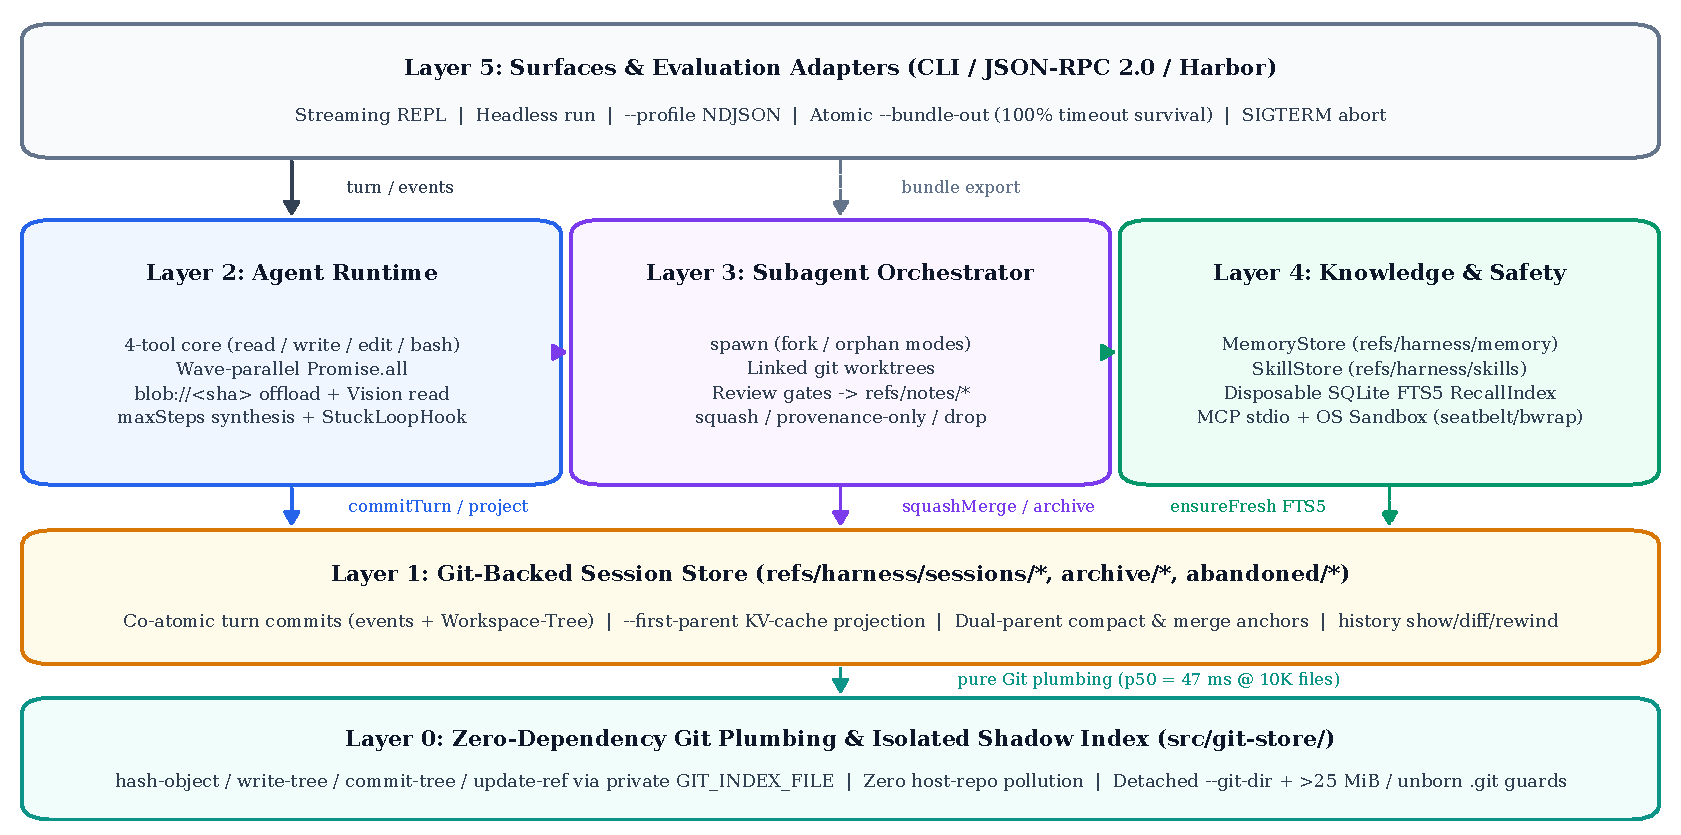
\includegraphics[width=\linewidth]{fig_architecture.pdf}
\caption{\textbf{Six-layer architecture of \texttt{git-harness}.} Lower layers never import higher layers; Layers~3--4 plug into Layer~2 strictly via narrow \texttt{Tool} and \texttt{RuntimeHook} interfaces, keeping Turn-0 prompt overhead under $1{,}500$ tokens.}
\label{fig:architecture}
\end{figure}

\subsection{Architecture overview}
\label{sec:arch-overview}
\texttt{git-harness} separates \emph{information management} (Layers~0, 1, and~4) from \emph{computation management} (Layers~2 and~3) and \emph{interaction surfaces} (Layer~5).
Information management governs what enters L1 prompt context, how workspace snapshots and conversation events are committed atomically, and what survives compaction, rewind, or restart.
Computation management maps model tool calls onto wave-parallel local execution, sandboxed shell commands, and isolated Git-branched subagents.
The runtime has zero npm dependencies and runs natively on Node.js ($\ge 22.18$), using built-in \texttt{node:sqlite} for disposable FTS5 cold indexing and system \texttt{git} for all object and ref persistence.

\subsection{Information hierarchy and explicit state transitions}
\label{sec:state-hierarchy}
A single LLM call conditions only on fixed weights (L0) and its active token sequence (L1).
Figure~\ref{fig:state-hierarchy} maps \texttt{git-harness}'s external state across four explicit tiers separated by the token-visible boundary between L1 and L2/L3:
\begin{itemize}[leftmargin=*,nosep]
  \item \textbf{L0 (Model Weights):} Fixed at inference. Because commit trailers record model-agnostic conversation events, adapters (OpenAI-compatible, Anthropic, local vLLM/SGLang) can be swapped seamlessly mid-session.
  \item \textbf{L1 (Active Context):} A deterministic projection of \texttt{refs/harness/sessions/<id>} generated solely by walking \texttt{--first-parent} back to the newest \texttt{compact} anchor.
  \item \textbf{L2 (Ephemeral Working State):} Offloaded oversized tool outputs stored as immutable Git blobs (\texttt{blob://<sha>}), linked \texttt{git worktree} directories, and active subagent branches (\texttt{refs/harness/agents/*}). Values enter L1 only when explicitly read or summarized.
  \item \textbf{L3 (Durable Git Object DAG):} Co-atomic turn commits, archived and abandoned branches (\code{refs/harness/{archive,abandoned}/*}), persistent memory (\code{refs/harness/memory}), versioned skills (\code{refs/harness/skills}), Git review notes (\code{refs/notes/harness/reviews}), and a disposable SQLite FTS5 index rebuildable deterministically from Git objects.
\end{itemize}

\begin{figure}[!t]
\centering
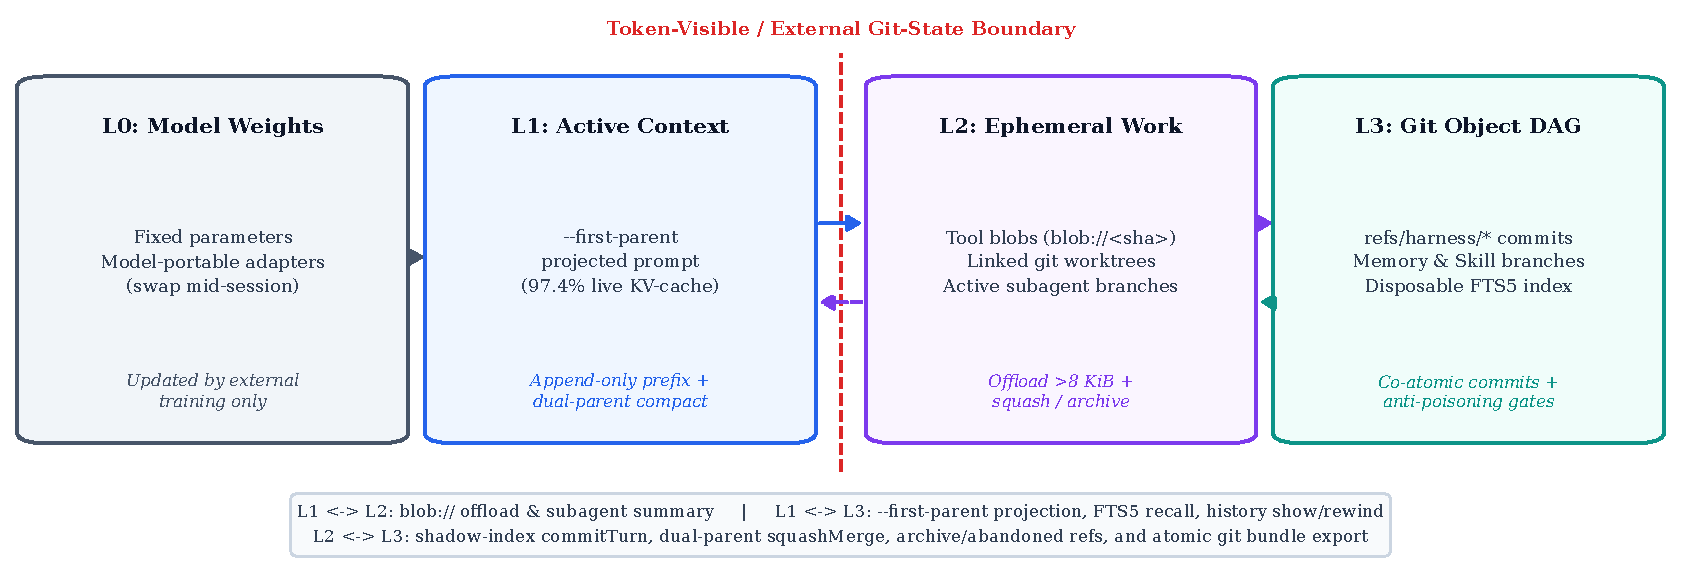
\includegraphics[width=\linewidth]{fig_state_hierarchy.pdf}
\caption{\textbf{Git-backed L0--L3 state hierarchy.} Explicit transitions move information across the L1/L2 boundary without mutating prior prompt prefixes or polluting the host repository.}
\label{fig:state-hierarchy}
\end{figure}

\subsection{Shadow-index plumbing, co-atomic DAG, and KV-cache invariance}
\label{sec:git-core}
\paragraph{Private shadow index (Layer 0).}
Standard Git commands mutate \texttt{.git/index} and \texttt{HEAD}, colliding with user staging areas and branches.
\texttt{GitCliStore} isolates all harness snapshots inside a private index file (\texttt{<gitDir>/harness-shadow.index}) passed via \texttt{GIT\_INDEX\_FILE}.
Snapshots execute \texttt{git add -A} and \texttt{git write-tree} in this private index without touching \texttt{.git/index} or \texttt{refs/heads/*}.
For non-Git workspaces (e.g., containerized benchmarks), detached \texttt{--git-dir /tmp/harness.git} mode provides full Git versioning with zero \texttt{.git} footprint in \texttt{/app}, guarding against nested unborn \texttt{.git} directories and automatically excluding compiled artifacts, VM disk images (\texttt{*.img}, \texttt{*.qcow2}, \texttt{*.iso}), and files exceeding $25\,\mathrm{MiB}$.
On read-only steps (\texttt{read}, \texttt{recall}, non-mutating \texttt{history}), Layer~0 skips workspace hashing and reuses the parent commit's \texttt{Workspace-Tree} SHA in $O(1)$ time ($\sim 3\text{--}8\,\mathrm{ms}$).

\paragraph{Co-atomic session commits (Layer 1).}
Every turn commit on \texttt{refs/harness/sessions/<id>} stores a tree containing \texttt{turn/events.jsonl}, \texttt{turn/state.json}, \texttt{workspace/} (the exact post-step working tree), and \texttt{summary.md} (on \texttt{compact} and \texttt{subagent-merge} commits), annotated with structured Git trailers (\texttt{Harness-Kind}, \texttt{Agent-Id}, \texttt{Model}, \texttt{Tokens-In}, \texttt{Tokens-Out}, \texttt{Cache-Read}, \texttt{Workspace-Tree}).
Because conversation and files share one immutable commit, \texttt{history(\{action:"rewind", targetSha\})} atomically restores both while preserving the abandoned branch under \texttt{refs/harness/abandoned/*}.

\begin{theorem}[First-Parent KV-Cache Prefix Invariance]
Let $H_t$ be the tip of \code{refs/harness/sessions/<id>} after step $t$, and let $\Pi(H_t)$ be the message list produced by walking \texttt{git} \texttt{rev-list} \texttt{--first-parent} from $H_t$ back to the nearest \texttt{Harness-Kind: compact} ancestor (or root). For every non-compacting step $t \to t+1$---including steps that spawn, squash-merge, or drop arbitrary subagents via \texttt{parent2}---$\Pi(H_t)$ is a byte-identical prefix of $\Pi(H_{t+1})$.
\end{theorem}

\begin{proof}[Proof Sketch]
Turn commits set \texttt{parent1} $= H_t$ and append only new events; \texttt{subagent-merge} commits set \texttt{parent1} $= H_t$ and \texttt{parent2} $= S_{\text{tip}}$. Because $\Pi$ traverses only \texttt{parent1} and existing Git commits are immutable, earlier serialized messages never change, guaranteeing maximal prefix reuse on inference engines supporting KV-cache prefix caching.
\end{proof}

\subsection{Wave-parallel runtime, \texttt{blob://} offloading, and subagent orchestration}
\label{sec:runtime-orch}
\paragraph{Minimal 4-tool runtime (Layer 2).}
Layer~2 exposes four core tools (\texttt{read}, \texttt{write}, \texttt{edit}, \texttt{bash}) with wave-parallel execution: contiguous read-only or parallel-safe tool calls (\texttt{read}, \texttt{recall}, \texttt{subagent}) run concurrently via \texttt{Promise.all} with deterministic output ordering, while mutating calls act as ordering barriers.
The \texttt{read} tool handles UTF-8 line ranges, native multimodal image attachments (\texttt{.png}, \texttt{.jpg}, \texttt{.webp}, \texttt{.gif}), historical commit files (\texttt{commit://<sha>/<path>}), skills (\texttt{skill://<name>/SKILL.md}), and offloaded blobs (\texttt{blob://<sha>}).
Any tool output exceeding a threshold ($8\,\mathrm{KiB}$ default for \texttt{bash}) is stored directly via \texttt{git hash-object -w} and replaced in L1 with a head+tail preview plus a \texttt{blob://<sha>} pointer---combining lossless observation masking~\citep{lindenbauer2025complexity} with on-demand exact retrieval.

\paragraph{Git-native subagent lifecycle (Layer 3).}
\texttt{SubagentOrchestrator} implements \texttt{spawn} $\to$ \texttt{run} $\to$ \texttt{review} $\to$ \texttt{integrate}:
\begin{enumerate}[leftmargin=*,nosep]
  \item \textbf{Spawn:} Creates \texttt{refs/harness/agents/<id>} in \texttt{fork} mode (inheriting parent context) or \texttt{orphan} mode (\texttt{parents=[]}), optionally provisioning a linked \texttt{git worktree} seeded with the parent's uncommitted \texttt{Workspace-Tree}.
  \item \textbf{Run:} Executes either a native \texttt{RuntimeAgentRunner} or any external CLI (\texttt{ExternalCliRunner}) under a single runner interface.
  \item \textbf{Review:} Runs shell verification gates inside the subagent's worktree and stores structured verdicts in \texttt{refs/notes/harness/reviews}.
  \item \textbf{Integrate:} Serialized via a per-session lock to prevent CAS ref races across parallel workers. Supports \texttt{squash} (3-way conflict check + dual-parent \texttt{subagent-merge}, with optional \texttt{applyWorkspaceChanges: false} for provenance-only research merges), \texttt{cherry-pick}, or \texttt{drop} (archiving the tip under \texttt{refs/harness/archive/agents/<id>}).
\end{enumerate}

\subsection{Disposable FTS5 cold recall and gated memory/skills}
\label{sec:knowledge}
Persistent project memory (\texttt{refs/harness/memory}) and versioned skills (\texttt{refs/harness/skills}) reside on dedicated orphan Git branches.
Every proposed update passes deterministic pre-commit promotion gates (rejecting leaked API keys, private keys, malformed frontmatter, or oversized files) and records \texttt{parent2} provenance back to the originating session commit---directly mitigating memory poisoning and contaminated skill persistence~\citep{karten2026primeagent}.
Cold retrieval is served by \texttt{RecallIndex}, a disposable SQLite FTS5 index over all harness refs that can be wiped and deterministically rebuilt from Git objects at any time.

\subsection{Long-horizon invariants, guardrails, and forensic accounting}
\label{sec:invariants}
Running \texttt{git-harness} on hundreds of long-horizon tasks surfaced three operational invariants enforced directly by Layers~1--5:

\begin{invariant}[Graceful Synthesis Handoff on \texttt{maxSteps}]
Action step budgets must be decoupled from final handoff synthesis. When an agent or subagent reaches \texttt{steps == maxSteps} mid-tool-loop, hard-stopping leaves \texttt{assistantText} containing pre-tool narration while discarding verified findings. \texttt{git-harness} executes one final tool-disabled (\texttt{tools=[]}) synthesis call, commits it to the branch, and reports \texttt{stopReason: "max\_steps"} explicitly to the caller.
\end{invariant}

\begin{invariant}[Lossless Cold-Storage Completeness]
Archiving or rewinding removes a branch from hot \texttt{--first-parent} projection, never from cold search. \texttt{RecallIndex} indexes all refs under \code{refs/harness/{sessions,agents,archive,abandoned}/*} plus \code{refs/harness/memory}. Before every \texttt{recall} query, \texttt{ensureFresh()} compares an $O(|\text{refs}|)$ fingerprint of \texttt{(ref, sha)} tips and rebuilds only when any Git ref changed. Moreover, \texttt{history(\{action:"show", targetSha\})} makes every SHA or archive ref directly inspectable.
\end{invariant}

\begin{invariant}[Monotonic Oscillation Guardrails \& Timeout Forensics]
Sliding-window file-churn detectors silently stall once repeated edits saturate window size $W$ with $W \bmod k \neq 0$. \texttt{StuckLoopHook} pairs sliding-window density with a monotonic per-path edit counter ($c \bmod k = 0$) plus step-budget and optional wall-clock \texttt{timeBudgetMs} notices. To preserve forensics on hard timeouts, \texttt{--bundle-out} atomically refreshes \texttt{session.bundle} on commit~1, every 10 commits, compaction, \texttt{SIGTERM}, and exit.
\end{invariant}

% ======================================================================
\section{Evaluation}
\label{sec:evaluation}
% ======================================================================

Our evaluation addresses three research questions derived directly from \texttt{git-harness}'s design:
\begin{itemize}[leftmargin=*,nosep]
  \item \textbf{RQ1 (Overhead \& Prefix Economics):} Does native Git plumbing scale to large repositories at sub-percent overhead while delivering statistically significant KV-cache efficiency on real long-horizon tasks?
  \item \textbf{RQ2 (Causal Component Attribution):} Which harness mechanisms (\texttt{blob://} offloading, \texttt{StuckLoopHook}, \texttt{subagent} delegation) causally improve accuracy, latency, and cost—and which introduce friction?
  \item \textbf{RQ3 (Forensic Harness Evolution \& Trajectory Analysis):} How do portable \texttt{session.bundle} DAGs turn opaque failures into deterministic engineering fixes, and what do real unpacked trajectories reveal?
\end{itemize}

Following recent agent-evaluation rigor standards~\citep{kapoor2026hal,zhu2025abc}, we report paired non-parametric significance tests (exact two-sided McNemar, paired Wilcoxon signed-rank), $10{,}000$-resample bootstrap confidence intervals, full failure taxonomies, and cache-weighted API cost ($10{:}1$ prompt-cache pricing: $\$3$/1M uncached input, $\$0.30$/1M cached input, $\$15$/1M output).

\subsection{RQ1: Scaling microbenchmarks, controlled ablations, and full 89-task sweep}
\label{sec:rq1}

\paragraph{Repository scaling ($100 \to 20{,}000$ files).}
Table~\ref{tab:latency} and Figure~\ref{fig:scaling} measure \texttt{GitCliStore} + \texttt{SessionStore} across five repository scales (plus $500$ ignored files) with workspace mutations on every turn.
Even at $20{,}000$ tracked files, median \texttt{commitTurn} latency stays at $66.2\,\mathrm{ms}$ ($p_{95}=92.9\,\mathrm{ms}$, under our $100\,\mathrm{ms}$ P0-6 target), while warm \texttt{project(HEAD)} stays flat at $0.1\,\mathrm{ms}$ independent of repository size.

\begin{table}[!t]
\centering
\caption{Git shadow-index latency scaling ($100$ to $20{,}000$ tracked files + $500$ ignored files).}
\label{tab:latency}
\small
\begin{tabular}{@{}rrrrr@{}}
\toprule
\textbf{Tracked Files ($N$)} & \textbf{\texttt{commitTurn} p50} & \textbf{\texttt{commitTurn} p95} & \textbf{\texttt{project} Warm} & \textbf{\texttt{project} Cold (21 msgs)} \\
\midrule
$100$      & $28.2\,\mathrm{ms}$ & $50.8\,\mathrm{ms}$ & $0.1\,\mathrm{ms}$ & $11.3\,\mathrm{ms}$ \\
$1{,}000$  & $30.9\,\mathrm{ms}$ & $55.1\,\mathrm{ms}$ & $0.1\,\mathrm{ms}$ & $12.8\,\mathrm{ms}$ \\
$5{,}000$  & $36.7\,\mathrm{ms}$ & $60.3\,\mathrm{ms}$ & $0.1\,\mathrm{ms}$ & $12.8\,\mathrm{ms}$ \\
$10{,}000$ & $47.3\,\mathrm{ms}$ & $72.7\,\mathrm{ms}$ & $0.1\,\mathrm{ms}$ & $14.9\,\mathrm{ms}$ \\
$20{,}000$ & $66.2\,\mathrm{ms}$ & $92.9\,\mathrm{ms}$ & $0.1\,\mathrm{ms}$ & $14.3\,\mathrm{ms}$ \\
\bottomrule
\end{tabular}
\end{table}

\begin{figure}[!t]
\centering
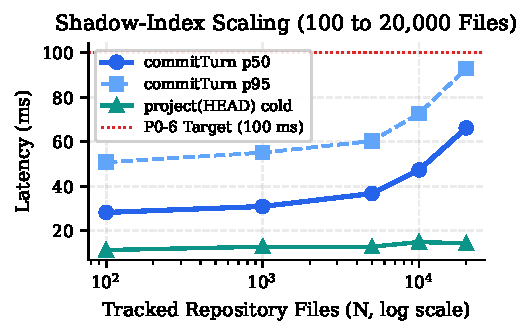
\includegraphics[width=0.62\linewidth]{fig_scaling.pdf}
\caption{\textbf{Shadow-index scaling.} Persistent \texttt{GIT\_INDEX\_FILE} \texttt{commitTurn} latency remains below $100\,\mathrm{ms}$ ($p_{95}$) at $20{,}000$ tracked files while \texttt{project(HEAD)} remains flat.}
\label{fig:scaling}
\end{figure}

\paragraph{Controlled P1 ablations (\texttt{npm run eval}).}
To isolate architectural mechanisms from LLM decoding variance, Table~\ref{tab:p1} reports four deterministic P1 rubric benchmarks against standard harness baselines.
All four pass with wide margins: active prompt size drops by $76.5\%$ vs.\ linear transcripts, multi-compaction KV-cache retention rises from $47.5\%$ (sliding window) to $91.0\%$, cold recall after three compactions jumps from $10\%$ to $100\%$, and subagent handoffs compress context to $3.0\%$ while keeping $100\%$ lossless \texttt{parent2} provenance.

\begin{table}[!t]
\centering
\caption{Controlled P1 ablation scorecard (\texttt{npm run eval}).}
\label{tab:p1}
\small
\begin{tabular}{@{}llcc@{}}
\toprule
\textbf{ID} & \textbf{Metric} & \textbf{\texttt{git-harness}} & \textbf{Baseline} \\
\midrule
\texttt{P1-POLLUTION} & Active Context Reduction & \textbf{$-76.5\%$} ($1{,}054$ ch) & $0.0\%$ ($4{,}489$ ch) \\
\texttt{P1-KVCACHE}   & KV-Cache Prefix Hit (25 turns + compact) & \textbf{$91.0\%$} & $47.5\%$ (sliding window) \\
\texttt{P1-RECALL}    & Cold Recall Precision (after 3 compactions) & \textbf{$100\%$} ($10/10$) & $10\%$ ($1/10$ active-only) \\
\texttt{P1-HANDOFF}   & Subagent Handoff Compression Ratio & \textbf{$3.0\%$} + \texttt{parent2} & $100\%$ (inline transcript) \\
\bottomrule
\end{tabular}
\end{table}

\paragraph{Clean full 89-task Terminal-Bench v2.1 sweeps.}
We evaluated three clean, independent full 89-task sweeps ($k=1$) on Terminal-Bench v2.1~\citep{merrill2026terminalbench} under an identical OpenAI-compatible reasoning model endpoint (\texttt{reasoning\_effort=high}, \texttt{max\_tokens=32768}), identical timeouts, and identical Harbor sandboxes ($-n\,16$, $-r\,2$): \texttt{pi v0.83.0}, baseline \texttt{git-harness v0.5}, and evolved \texttt{git-harness v0.7.1} (Table~\ref{tab:tb21main}, Figures~\ref{fig:kvcache} and~\ref{fig:cost}).

\begin{table}[!t]
\centering
\caption{Clean full 89-task Terminal-Bench v2.1 sweeps ($k=1$, identical reasoning model and timeouts).}
\label{tab:tb21main}
\resizebox{\linewidth}{!}{%
\begin{tabular}{@{}lccc@{}}
\toprule
\textbf{Metric} & \textbf{\texttt{pi v0.83.0}} & \textbf{\texttt{git-harness v0.5}} & \textbf{\texttt{git-harness v0.7.1}} \\
\midrule
Tasks Passed (Clean Full-Sweep Pass@1) & $76 / 89$ ($85.39\%$) & $70 / 89$ ($78.65\%$) & $72 / 89$ ($80.90\%$) \\
McNemar Exact Two-Sided $p$ vs.\ \texttt{pi} & --- & $p = 0.238$ ($6$ vs.\ $12$) & $p = 0.455$ ($6$ vs.\ $10$) \\
Failures (Logic / AgentTO / VerifTO / Crash) & $10$ / $2$ / $1$ / $0$ & $15$ / $2$ / $1$ / $1$ & $12$ / $4$ / $1$ / \textbf{$0$} \\
Agent Duration (Median / Mean) & $72.9\,\mathrm{s}$ / $231.2\,\mathrm{s}$ & $103.1\,\mathrm{s}$ / $356.7\,\mathrm{s}$ & $124.9\,\mathrm{s}$ / $366.5\,\mathrm{s}$ \\
Est.\ API Cost (Median / Mean, 10:1 cache) & $\$0.141$ / $\$0.282$ & $\$0.141$ / $\$0.483$ & $\$0.161$ / $\$0.519$ \\
Per-Task KV-Cache Hit (Mean / Median) & $86.19\%$ / $87.39\%$ & $86.88\%$ / $86.40\%$ & \textbf{$87.64\%$ / $88.78\%$} ($p=0.029$) \\
Weighted Live KV-Cache Hit Rate & $93.71\%$ & $97.35\%$ & \textbf{$97.40\%$} ($2.42\times$ less uncached) \\
Git Checkpoint Overhead (Med / Mean) & --- & $0.206\%$ / $1.162\%$ & \textbf{$0.176\%$ / $0.585\%$} \\
Portable \texttt{session.bundle} Survival & --- & $84/89$ ($73.4\,\mathrm{KB}$ med) & \textbf{$89/89$ ($100\%$, $62.9\,\mathrm{KB}$ med)} \\
\bottomrule
\end{tabular}}
\end{table}

\begin{figure}[!t]
\centering
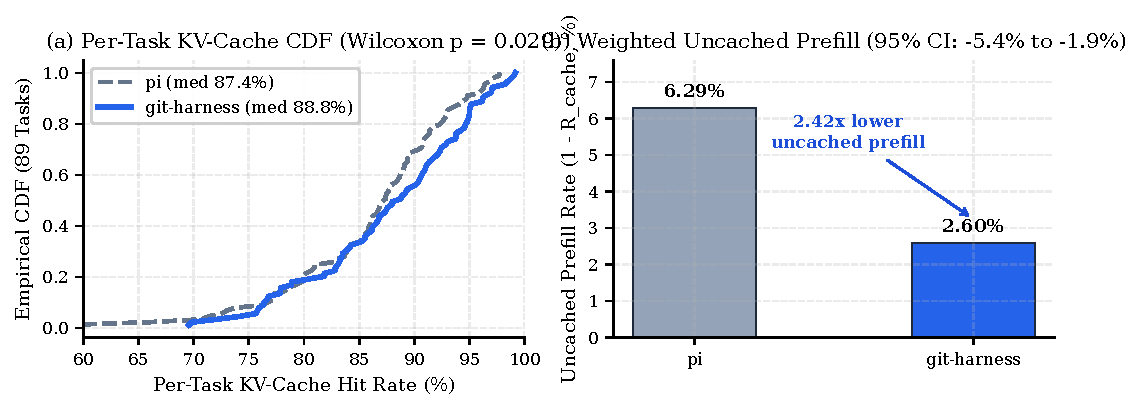
\includegraphics[width=\linewidth]{fig_kvcache.pdf}
\caption{\textbf{KV-cache efficiency across 89 Terminal-Bench v2.1 tasks.} (a) Empirical CDF of per-task KV-cache hit rate (paired Wilcoxon $p = 0.0289$); (b) weighted uncached prefill rate ($1 - R_{\text{cache}}$), showing a $2.42\times$ reduction in uncached prefill for \texttt{git-harness v0.7.1} (95\% cluster bootstrap CI on cache gain: $[+1.92\%, +5.42\%]$).}
\label{fig:kvcache}
\end{figure}

\begin{figure}[!t]
\centering
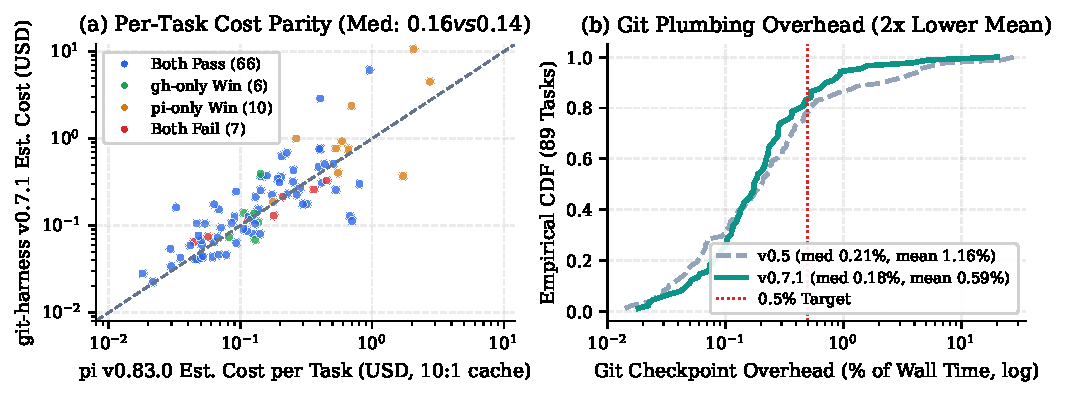
\includegraphics[width=\linewidth]{fig_cost_overhead.pdf}
\caption{\textbf{Cost parity and Git overhead across 89 tasks.} (a) Paired estimated API cost under 10:1 cache pricing (median $\$0.16$ vs.\ $\$0.14$); (b) empirical CDF of Git checkpoint overhead (\% wall time), showing $2\times$ lower mean overhead in \texttt{v0.7.1} ($0.59\%$ vs.\ $1.16\%$) and median $0.18\%$.}
\label{fig:cost}
\end{figure}

Three quantitative conclusions stand out:
\begin{enumerate}[leftmargin=*,nosep]
  \item \textbf{Accuracy parity with zero harness crashes:} \texttt{git-harness v0.7.1} improves clean Pass@1 from $70/89$ to $72/89$ ($80.90\%$), statistically indistinguishable from \texttt{pi v0.83.0} ($76/89$, McNemar exact $p = 0.4545$). Deterministic harness crashes dropped $1 \to 0$, and logic failures dropped $15 \to 12$.
  \item \textbf{Statistically significant KV-cache advantage:} Per-task KV-cache hit rate beats \texttt{pi} by $+1.45\%$ mean (95\% bootstrap CI $[+0.04\%, +2.85\%]$, Wilcoxon $p = 0.0289$). Weighted across all input tokens, \texttt{git-harness v0.7.1} reaches $97.40\%$ vs.\ $93.71\%$ (95\% cluster bootstrap CI $[+1.92\%, +5.42\%]$), reducing the uncached prefill rate by \textbf{$2.42\times$} ($6.29\% \to 2.60\%$).
  \item \textbf{Sub-percent overhead and $100\%$ bundle survival:} Mean Git overhead halved from \texttt{v0.5} to \texttt{v0.7.1} ($1.162\% \to 0.585\%$, median $0.176\%$), median bundle size shrank to $62.9\,\mathrm{KB}$, and $89/89$ trials preserved complete forensic bundles. Median API cost matches \texttt{pi} ($\$0.161$ vs.\ $\$0.141$), while mean cost ($\$0.519$ vs.\ $\$0.282$) isolates heavy-tail $100\text{--}300$-step runs—explaining why we next ablate individual runtime mechanisms.
\end{enumerate}

\subsection{RQ2: Live 4-arm causal component ablation (15 hard tasks)}
\label{sec:rq2}
To establish causal attribution on real tasks rather than relying on cross-version correlations, we selected the top 15 feature-active tasks ($<950\,\mathrm{s}$ in clean \texttt{v0.7.1}, objectively ranked by \texttt{subagent}, \texttt{blob://}, \texttt{history}, and \texttt{recall} counts) and toggled one mechanism off at a time under identical model, timeout, and sandbox settings: (1) \textbf{No \texttt{blob://} offload} (\texttt{--offload-bytes 0}), (2) \textbf{No \texttt{StuckLoopHook}} (\texttt{--no-stuck-hook}), and (3) \textbf{No \texttt{subagent}} (\texttt{--no-subagents}). Table~\ref{tab:ablation} and Figure~\ref{fig:ablation} report all five arms alongside \texttt{pi v0.83.0}.

\begin{table}[!t]
\centering
\caption{Live 4-arm causal component ablation on the 15 most feature-active Terminal-Bench v2.1 tasks (plus \texttt{pi v0.83.0} reference). Costs include root + nested subagent tokens under 10:1 cache pricing.}
\label{tab:ablation}
\resizebox{\linewidth}{!}{%
\begin{tabular}{@{}lcccccc@{}}
\toprule
\textbf{Configuration} & \textbf{Pass@1} & \textbf{Timeouts} & \textbf{Med / Mean Dur} & \textbf{W-KV-Cache} & \textbf{Med / Mean Cost} & \textbf{Total Cost} \\
\midrule
\texttt{pi v0.83.0} (reference) & $12/15$ ($80.0\%$) & $1$ & $144.4\,\mathrm{s}$ / $367.8\,\mathrm{s}$ & $91.86\%$ & $\$0.253$ / $\$0.307$ & $\$4.60$ \\
Full \texttt{git-harness v0.7.1} & $11/15$ ($73.3\%$) & $0$ & $404.1\,\mathrm{s}$ / $417.7\,\mathrm{s}$ & $96.16\%$ & $\$0.442$ / $\$0.651$ & $\$9.76$ \\
\quad $-$ No \texttt{blob://} offload & $10/15$ ($66.7\%$) & \textbf{$3$} & $419.9\,\mathrm{s}$ / \textbf{$795.4\,\mathrm{s}$} & $96.69\%$ & \textbf{$\$0.571$} / \textbf{$\$0.904$} & \textbf{$\$13.56$} \\
\quad $-$ No \texttt{StuckLoopHook} & $10/15$ ($66.7\%$) & \textbf{$2$} & $429.7\,\mathrm{s}$ / \textbf{$561.3\,\mathrm{s}$} & $96.85\%$ & $\$0.350$ / $\$0.678$ & $\$10.17$ \\
\quad $-$ No \texttt{subagent} (Git core) & \textbf{$14/15$ ($93.3\%$)} & \textbf{$0$} & $296.5\,\mathrm{s}$ / $470.9\,\mathrm{s}$ & \textbf{$97.76\%$} & \textbf{$\$0.201$} / $\$0.649$ & $\$9.73$ \\
\bottomrule
\end{tabular}}
\end{table}

\begin{figure}[!t]
\centering
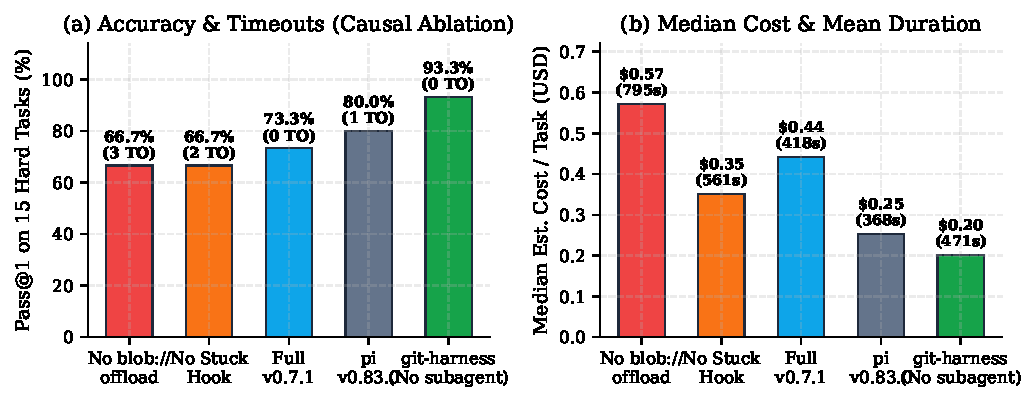
\includegraphics[width=\linewidth]{fig_ablation.pdf}
\caption{\textbf{Live 4-arm causal ablation on 15 hard Terminal-Bench v2.1 tasks.} Removing \texttt{blob://} offloading or \texttt{StuckLoopHook} triggers container timeouts and $+34\%\text{--}+90\%$ duration increases, whereas disabling eager Turn-0 \texttt{subagent} delegation raises Pass@1 to $14/15$ ($93.3\%$) and cuts median cost by $55\%$.}
\label{fig:ablation}
\end{figure}

Three causal findings emerge:
\begin{enumerate}[leftmargin=*,nosep]
  \item \textbf{\texttt{blob://} offloading is causally protective:} Disabling it nearly doubled mean wall time ($417.7\,\mathrm{s} \to 795.4\,\mathrm{s}$, $+90.4\%$), raised total API cost $+39\%$ ($\$9.76 \to \$13.56$), lowered Pass@1 ($11/15 \to 10/15$), and caused $3$ container timeouts (\texttt{feal-linear-cryptanalysis}, \texttt{rstan-to-pystan}, \texttt{regex-chess})---confirming observation masking's real-world leverage~\citep{lindenbauer2025complexity}.
  \item \textbf{\texttt{StuckLoopHook} prevents runaway trajectories:} Disabling failure-streak and file-churn guardrails increased mean duration $+34.4\%$ ($417.7\,\mathrm{s} \to 561.3\,\mathrm{s}$), dropped Pass@1 ($11/15 \to 10/15$), and caused $2$ runaway timeouts (\code{sanitize-git-repo} $49\,\mathrm{s} \to 900\,\mathrm{s}$; \code{llm-inference-batching-scheduler} $807\,\mathrm{s} \to 1800\,\mathrm{s}$).
  \item \textbf{The Subagent Over-Delegation Tax:} Crucially, disabling the always-on \texttt{subagent} tool---while retaining \texttt{git-harness}'s Git core (shadow index, \texttt{blob://}, \texttt{StuckLoopHook}, \texttt{history}, \texttt{recall})---jumped Pass@1 from $11/15$ to \textbf{$14/15$ ($93.3\%$)}, surpassing \texttt{pi v0.83.0} ($12/15$) with $0$ timeouts, raising weighted KV-cache hit rate to \textbf{$97.76\%$} ($3.63\times$ lower uncached prefill than \texttt{pi}'s $91.86\%$), and cutting median per-task cost by \textbf{$55\%$} ($\$0.442 \to \$0.201$, $21\%$ cheaper than \texttt{pi}'s $\$0.253$). On individual tasks, removing eager subagents cut wall time dramatically (\code{feal-linear-cryptanalysis} $876\,\mathrm{s} \to 79\,\mathrm{s}$; \code{llm-inference-batching-scheduler} $807\,\mathrm{s} \to 92\,\mathrm{s}$; \code{db-wal-recovery} $163\,\mathrm{s} \to 12\,\mathrm{s}$). This quantitatively confirms Prime Agent's qualitative observation that current models struggle to allocate subagents~\citep{karten2026primeagent}, yielding a concrete design rule: \emph{subagent delegation should be escalation-triggered rather than eagerly prompted on Turn~0.}
\end{enumerate}

\subsection{RQ3: Forensic harness evolution and trajectory case studies}
\label{sec:rq3}

\paragraph{Deterministic fixes driven by \texttt{session.bundle} forensics (\texttt{v0.5} $\to$ \texttt{v0.7.1}).}
Unpacking \texttt{session.bundle} DAGs and \texttt{profile.jsonl} logs across failed runs exposed concrete harness bugs rather than prompting guesswork:
\begin{itemize}[leftmargin=*,nosep]
  \item \textbf{\texttt{v0.5} $\to$ \texttt{v0.6}:} Guarding unborn nested \texttt{.git} repos fixed an instant $2\,\mathrm{s}$ crash on \code{merge-diff-arc-agi-task} (PASS in $162.9\,\mathrm{s}$ in full \texttt{v0.7.1}); adding multimodal image \texttt{read} flipped \code{chess-best-move} to PASS in $39.4\,\mathrm{s}$ ($4.2\times$ faster than \texttt{pi}'s $166\,\mathrm{s}$); raising default \texttt{bash} timeout ($30\,\mathrm{s} \to 120\,\mathrm{s}$) fixed premature test kills on \code{regex-chess}; and excluding VM disk images compressed \code{qemu-alpine-ssh} bundles from $968\,\mathrm{MB} \to 12.0\,\mathrm{KB}$ ($21.99\% \to 0.05\%$ Git overhead).
  \item \textbf{\texttt{v0.6} $\to$ \texttt{v0.7}:} Inspecting \texttt{feal-differential-cryptanalysis} ($1440\,\mathrm{s}$ in \texttt{v0.5}) revealed an orphan subagent that solved the differential attack, hit \texttt{maxSteps} mid-tool-call, returned pre-tool narration, and archived under \texttt{refs/harness/archive/agents/*} (invisible to \texttt{RecallIndex}). Implementing Invariants~1--2 sped up \texttt{feal-differential-cryptanalysis} by $6.6\times\text{--}7.8\times$ ($1440\,\mathrm{s} \to 185.1\,\mathrm{s}$ targeted / $216.6\,\mathrm{s}$ full sweep, $18.3\,\mathrm{KB}$ bundle) and raised \texttt{history} tool adoption $9\times$ ($2 \to 18$ calls across 89 tasks).
  \item \textbf{\texttt{v0.7} $\to$ \texttt{v0.7.1}:} Auditing \texttt{gpt2-codegolf} ($61$ edits to \texttt{gpt2.c}, \texttt{bundle=NONE} on timeout) exposed the file-churn modulo dead-zone and missing timeout bundle export. Fixing both yielded $89/89$ ($100\%$) bundle survival and flipped \texttt{gpt2-codegolf} to PASS in the clean full sweep.
\end{itemize}

\paragraph{Methodological lesson: targeted re-runs vs.\ clean full sweeps.}
During development, targeted failure re-runs recovered $11$ previously failing tasks (a multi-run union of $81/89 = 91.01\%$).
Yet our unconditioned full 89-task \texttt{v0.7.1} sweep scored $72/89$ ($80.90\%$): $+7$ tasks flipped $\text{FAIL}\to\text{PASS}$ (\texttt{break-filter-js-from-html}, \texttt{chess-best-move}, \texttt{crack-7z-hash}, \texttt{gcode-to-text}, \texttt{gpt2-codegolf}, \texttt{merge-diff-arc-agi-task}, \texttt{model-extraction-relu-logits}), while $5$ previously passing tasks saw stochastic $k=1$ flips (two-sweep union $77/89 = 86.52\%$).
Reporting both transparently illustrates why targeted re-runs verify deterministic bug fixes, whereas only clean full sweeps with paired statistical tests avoid selection-bias inflation.

\paragraph{Unpacked DAG case studies.}
Appendix~\ref{app:traces} reproduces real unpacked commit graphs from \texttt{session.bundle}:
(1) \textbf{\texttt{winning-avg-corewars}} demonstrates three concurrent isolated subagents (\texttt{strategy-a/b/c}) consuming $1.18\mathrm{M}$ worker tokens across separate branches before merging via three dual-parent \texttt{subagent-merge} commits (\texttt{869c43da}, \texttt{64a967aa}, \texttt{42c612eb}), keeping parent context under $13.5\mathrm{K}$ tokens; and
(2) \textbf{\texttt{path-tracing-reverse}} demonstrates $243$ steps ($247$ commits) maintaining $99.3\%$ live KV-cache hit rate, committing a dual-parent compaction anchor (\texttt{c5a8756c}) at Step~224 that drops context from $160.0\mathrm{K} \to 1.5\mathrm{K}$ tokens, followed by $2\text{--}4\,\mathrm{ms}$ FTS5 \texttt{recall} queries on Steps~239 and~241.

% ======================================================================
\section{Related Work}
\label{sec:related}
% ======================================================================

\paragraph{Coding agent harnesses and harness engineering.}
SWE-agent~\citep{yang2024sweagent} formalized Agent-Computer Interfaces (ACIs), while OpenHands~\citep{wang2024openhands,openhands2025sdk} introduced a modular event-stream runtime and SDK.
Recent empirical work formalizes harness engineering as a first-class discipline~\citep{barbaste2026harness,ning2026codeasharness}, quantifies how harness evolution shapes benchmark accuracy on fixed models~\citep{sghaier2026dontblame}, and explores automated harness synthesis~\citep{lou2026autoharness,lee2026metaharness,lin2026agenticharness}.
Most closely related is \textbf{Prime Agent}~\citep{karten2026primeagent}, which integrates a persistent IPython REPL (RLM abstraction), async recursive subagents with message queues, and a typed Continual Harness over custom disk persistence.
Whereas Prime Agent prioritizes maximum programmatic expressivity (and notes friction with irreversible actions and contaminated online skill refinements on Factorio), \texttt{git-harness} prioritizes a minimal, zero-dependency \emph{native Git substrate} delivering co-atomic conversation+workspace rewind, pre-commit anti-poisoning gates, and formally prefix-invariant KV-cache economics (Table~\ref{tab:compare}).

\begin{table}[!t]
\centering
\caption{Architectural comparison of \texttt{git-harness} against contemporary coding agent harnesses.}
\label{tab:compare}
\resizebox{\linewidth}{!}{%
\begin{tabular}{@{}lccccc@{}}
\toprule
\textbf{Capability} & \textbf{\texttt{git-harness}} & \textbf{Prime Agent} & \textbf{GCC} & \textbf{OpenHands} & \textbf{\texttt{pi v0.83}} \\
\midrule
Storage substrate & Native Git plumbing & Custom disk/daemon & \texttt{.GCC/} MD & Event log + FS & JSONL \\
Co-atomic chat + FS rewind & \textbf{Yes (1 commit)} & Separate & Partial & No & No \\
Zero host-repo pollution & \textbf{Yes (shadow idx)} & N/A & No (\texttt{.GCC/}) & Container & N/A \\
KV-cache prefix invariance & \textbf{Formal (\texttt{-1st-par})} & Unanalyzed & No & Partial & Append-only \\
Multi-agent provenance & \textbf{\texttt{parent2} + notes} & Queue tree & Manual merge & Sub-events & None \\
Pre-commit memory gates & \textbf{Yes (anti-secret)} & Unvalidated & No & No & N/A \\
Portable single-file trace & \textbf{\texttt{git bundle}} & Log dir & Dir & Log dir & JSONL \\
\bottomrule
\end{tabular}}
\end{table}

\paragraph{Git-based agent state and memory.}
Git Context Controller (GCC)~\citep{wu2025gcc} models agent memory using Git metaphors (\texttt{COMMIT}, \texttt{BRANCH}, \texttt{MERGE}) inside a bespoke \texttt{.GCC/} markdown directory, and EvoGit~\citep{evogit2025} coordinates decentralized code evolution through a Git phylogenetic graph.
\texttt{git-harness} goes beyond Git metaphors by executing directly on Git's content-addressed object database, private shadow indices, linked worktrees, and notes to unify sessions, workspace snapshots, blob offloading, subagents, memory, and skills without touching user branches.

\paragraph{Context compression and KV-cache economics.}
ACE~\citep{zhang2026ace} evolves itemized context playbooks to prevent context collapse, while Lindenbauer et al.~\citep{lindenbauer2025complexity} show that simple observation masking matches LLM summarization at lower cost.
\texttt{git-harness}'s \texttt{blob://<sha>} offloading combines lossless observation masking with content-addressed retrieval, and our \texttt{--first-parent} projection theorem guarantees prefix stability purely at the harness layer across any provider supporting prefix caching.

\paragraph{Evaluation rigor for coding agents.}
Terminal-Bench~\citep{merrill2026terminalbench} provides realistic containerized CLI tasks, while HAL~\citep{kapoor2026hal} and the Agentic Benchmark Checklist (ABC)~\citep{zhu2025abc} establish standards for cost-normalized evaluation, paired significance testing, and transparent selection-bias reporting---practices we apply throughout Section~\ref{sec:evaluation}.

% ======================================================================
\section{Conclusion}
\label{sec:conclusion}
% ======================================================================

Treating Git as a first-class runtime substrate collapses five fragmented agent-harness subsystems into a single, zero-dependency, content-addressed architecture.
Across 100--20,000-file microbenchmarks, controlled P1 ablations, clean 89-task Terminal-Bench v2.1 sweeps, and a 4-arm live causal ablation, \texttt{git-harness} demonstrates that co-atomic shadow-index commits, \texttt{--first-parent} KV-cache projection, \texttt{blob://} observation offloading, monotonic stuck-loop guardrails, and \texttt{git bundle} forensics jointly deliver high KV-cache efficiency ($97.40\%$, $p = 0.0289$), sub-percent plumbing overhead ($0.176\%$ median), and $100\%$ forensic reproducibility.
At the same time, our causal ablation reveals that current frontier models suffer an \emph{over-delegation tax} when subagent tools are eagerly promoted on Turn~0 ($11/15 \to 14/15$ Pass@1 and $-55\%$ median cost when disabling eager subagents).
Looking ahead, combining \texttt{git-harness}'s co-atomic Git governance substrate with escalation-triggered subagent allocation, persistent L2 REPL state, and gate-verified trajectory refinement (\texttt{/refine}) offers a principled path toward self-improving harnesses that remain fast, auditable, and safe.

\bibliographystyle{plainnat}
\bibliography{references}

% ======================================================================
\appendix
\section{Unpacked \texttt{session.bundle} Forensic Traces}
\label{app:traces}

Every Terminal-Bench v2.1 run exports a portable Git bundle (\texttt{session.bundle}) inspectable with standard Git commands. Below are exact excerpts from three real runs discussed in Section~\ref{sec:rq3}.

\paragraph{A.1 Parallel Subagent Squash-Merge DAG (\texttt{winning-avg-corewars}).}
On Step~2, the parent spawned three concurrent worktree subagents (\texttt{strategy-a/b/c}) consuming $1.18\mathrm{M}$ worker tokens before serializing three dual-parent \texttt{subagent-merge} commits onto \texttt{refs/harness/sessions/main}:
\begin{lstlisting}
$ git log --all --graph --oneline --decorate
* 23a0d7c0 (refs/harness/sessions/main) Step 8 (13.5K tok, PASS)
* ... (Steps 3..7)
* 246a9550 Step 2 (4.8K tok)
*   42c612eb squash(strategy-c) [parents: 64a967aa, 24638448]
|\
| * 24638448 (refs/harness/agents/strategy-c) 525.5K worker tok
* |   64a967aa squash(strategy-a) [parents: 869c43da, fca59711]
|\ \
| * | fca59711 (refs/harness/agents/strategy-a) 623.4K worker tok
* | |   869c43da squash(strategy-b) [parents: 2f029c58, cb453b26]
|\ \ \
| * | | cb453b26 (refs/harness/agents/strategy-b) 32.8K worker tok
|/ / /
* 2f029c58 Step 1 (1.4K tok)
\end{lstlisting}
Walking \texttt{git rev-list --first-parent refs/harness/sessions/main} traverses only \texttt{2f029c58} $\to$ \texttt{869c43da} $\to$ \texttt{64a967aa} $\to$ \texttt{42c612eb} $\to$ \texttt{246a9550} $\to \dots \to$ \texttt{23a0d7c0}, excluding all $1.18\mathrm{M}$ worker tokens from the parent KV-cache.

\paragraph{A.2 Dual-Parent Auto-Compaction + Cold Recall (\texttt{path-tracing-reverse}).}
At Step~224 (\texttt{0e7f13ce}), active prompt context reached $160.0\mathrm{K}$ tokens ($99.3\%$ cumulative KV-cache hit rate). Layer~1 committed compaction anchor \texttt{c5a8756c}, resetting Step~225 (\texttt{a47a34b9}) to $1.5\mathrm{K}$ tokens; Steps~239 (\texttt{1bb9175c}) and~241 (\texttt{006dd921}) then queried SQLite FTS5 \texttt{recall} in $4\,\mathrm{ms}$ and $2\,\mathrm{ms}$ to recover archived pre-compaction details:
\begin{lstlisting}
0e7f13ce  turn     Step 224  in=160.0K  cache=159.7K  wtree=a81862f4
c5a8756c  compact  Anchor    in=159.7K  parent1=0e7f13ce  (160.0K -> 1.5K)
a47a34b9  turn     Step 225  in=  1.5K  cache=  1.1K  wtree=a81862f4
1bb9175c  turn     Step 239  in= 11.1K  cache= 10.0K  tool=recall (4ms, 1839B)
006dd921  turn     Step 241  in= 13.0K  cache= 11.8K  tool=recall (2ms,  409B)
5b0cbef8  turn     Step 243  in= 13.7K  cache= 13.3K  PASS
\end{lstlisting}

\paragraph{A.3 Orphan Subagent Handoff Fix (\texttt{feal-differential-cryptanalysis}).}
In \texttt{v0.5}, an orphan subagent (\texttt{3a083e91}) hit \texttt{maxSteps} immediately after writing \texttt{/tmp/feal\_attack\_final.py}, returning pre-tool narration while archiving at \texttt{refs/harness/archive/agents/sub-1795640867844-1} (unindexed by \texttt{RecallIndex}); the parent spent $1440\,\mathrm{s}$ ($54$ steps) re-deriving the attack. After implementing Invariants~1--2 in \texttt{v0.7}, the archived subagent (\texttt{6a775588}) returned the complete differential derivation plus direct inspection hints (\texttt{history show 6a775588} / auto-refreshed \texttt{recall}), cutting total runtime to $185.1\,\mathrm{s}$ ($19$ steps; $216.6\,\mathrm{s}$ / $10$ steps in the clean \texttt{v0.7.1} full sweep).

\section{LLM Usage Disclosure}
Large language models assisted with implementation, benchmark automation, and manuscript formatting. All experimental protocols, statistical analyses, architectural claims, and empirical measurements were executed and verified directly against real test suites and Terminal-Bench v2.1 runs.

\end{document}
